\documentclass[12pt, titlepage]{article}
\usepackage{gensymb}
\usepackage{booktabs}
\usepackage{tabularx}
\usepackage{hyperref}
\usepackage{enumerate}
\usepackage{float} 
\usepackage{graphicx}
\hypersetup{
	colorlinks,
	citecolor=black,
	filecolor=black,
	linkcolor=blue,
	urlcolor=blue
}
\usepackage[round]{natbib}

\title{SE 3XA3: Test Plan\\Tetris Tussle}

\author{Nicholas Lobo \\ lobon3 \\ 400179304 \and
	Matthew Paulin \\ paulinm \\ 400187147 \and
	David Carrie \\ carriedd \\ 000661652 \and
}

\date{\today}



\begin{document}
	
	\maketitle
	
	\pagenumbering{roman}
	\tableofcontents
	\listoftables
	\listoffigures
	
	\begin{table}[bp]
		\caption{\bf Revision History}
		\begin{tabularx}{\textwidth}{p{3cm}p{2cm}X}
			\toprule {\bf Date} & {\bf Version} & {\bf Notes}\\
			\midrule
			2/26/2021 & 1.0 & Matthew, Nicolas and David initial work on the template\\
			2/28/2021 & 1.1 & Matthew, Nicolas and David completed section 3\\
			3/04/2021 & 1.3 & Matthew, Nicolas and David Completed Document for first submission.\\
			\bottomrule
		\end{tabularx}
	\end{table}
	
	\newpage
	
	\pagenumbering{arabic}
	
	
	\section{General Information}
	
	\subsection{Purpose}
	The purpose of testing our project is to verify that the form of satisfies the functions that are necessitated by the software requirements specification. Additionally, there may arise additional requirements that are discovered throughout the testing process.
	
	
	\subsection{Scope}
	The test plan is used to create methods by which the correctness and functionality of the project can be verified. This document will include what components of the project are being tested, for what purpose they are being tested, and how to test them. 
	\subsection{Acronyms, Abbreviations, and Symbols}
	
	\begin{table}[!htbp]
		\caption{\textbf{Table of Definitions}} \label{Table of Definitions}
		
		\begin{tabularx}{\textwidth}{p{3cm}X}
			\toprule
			\textbf{Term} & \textbf{Definition}\\
			\midrule
			\textbf{Tetromino} & A Tetromino is the geometric shape used in Tetris. It is composed of four squares connected at their edges to form 7 different shapes Definition1\\
			\bottomrule
		\end{tabularx}
		
	\end{table}	
	
	\subsection{Overview of Document}
	This document outlines the detailed testing plan that will be executed to give assurance that the system is behaving as stated in the requirements. It will lay out our plans for different types of testing including: acceptance, integration and unit testing as well as information regarding software tools to be used, personnel assignments, and scheduling.
	
	\section{Plan}
	
	\subsection{Software Description}
	The software being created is an updated and improved version of Tetris with multiplayer functionality and revised graphics.
	
	\subsection{Test Team}
	All group members currently working on the project will be part of the testing team. This includes:  Nicholas Lobo, Matthew Paulin, David Carrie.
	\subsection{Automated Testing Approach}
	All automated software tests will be completed through the use of the testing framework Jest.
	\subsection{Testing Tools}
	We will be using Jenkins to create a continuous integration testing environment and Jest to automate unit testing. Additionally, acceptance testing will be completed by some subset of the stakeholders to ensure that all the non functional requirements are sufficiently met.
	\subsection{Testing Schedule}
	
	See Gantt Chart at the following url ... (TO UPDATE LATER)
	
	\section{System Test Description}
	
	\subsection{Tests for Functional Requirements}
	
	\subsubsection{Controller Input Tests}
	\begin{enumerate}[{FR-CI-}1. ]
		\item
		\textbf{Type:} Dynamic, Manual
		
		\textbf{Initial State:} The user is in control of a Tetromino that is currently in play and in the middle of the board
		
		\textbf{Input:} The D key is pressed 
		
		\textbf{Output:} The Tetromino is shifted one board space to the right
		
		\textbf{How test will be performed:} The inputs will be pressed manually by the user and the output will be observed on the screen
		
		\item
		\textbf{Type:} Dynamic, Manual
		
		\textbf{Initial State:} The user is in control of a Tetromino that is currently in play and in the middle of the board
		
		\textbf{Input:} The A key is pressed 
		
		\textbf{Output:} The Tetromino is shifted one board space to the left
		
		\textbf{How test will be performed:} The inputs will be pressed manually by the user and the output will be observed on the screen
		
		\item
		\textbf{Type:} Dynamic, Manual
		
		\textbf{Initial State:} The user is in control of a Tetromino that is currently in play and in the middle of the board
		
		\textbf{Input:} The S key is pressed 
		
		\textbf{Output:} The Tetromino is shifted one board space down
		
		\textbf{How test will be performed:} The inputs will be pressed manually by the user and the output will be observed on the screen
		
		\item
		\textbf{Type:} Dynamic, Manual
		
		\textbf{Initial State:} The user is in control of a Tetromino that is currently in play and on the right edge of the board
		
		\textbf{Input:} The D key is pressed 
		
		\textbf{Output:} The Tetromino stays in the same position
		
		\textbf{How test will be performed:} The inputs will be pressed manually by the user and the output will be observed on the screen
		
		\item
		\textbf{Type:} Dynamic, Manual
		
		\textbf{Initial State:} The user is in control of a Tetromino that is currently in play and on the left edge of the board
		
		\textbf{Input:} The A key is pressed 
		
		\textbf{Output:} The Tetromino stays in the same position
		
		\textbf{How test will be performed:} The inputs will be pressed manually by the user and the output will be observed on the screen
		
		\item
		\textbf{Type:} Dynamic, Manual
		
		\textbf{Initial State:} The user is in control of a Tetromino that is currently in play and on the bottom edge of the board
		
		\textbf{Input:} The S key is pressed 
		
		\textbf{Output:} The Tetromino stays in the same position
		
		\textbf{How test will be performed:} The inputs will be pressed manually by the user and the output will be observed on the screen
		
		\item
		\textbf{Type:} Dynamic, Manual
		
		\textbf{Initial State:} The user is in control of a Tetromino that is currently in play and there is a Tetromino piece currently to the right of it.
		
		\textbf{Input:} The D key is pressed 
		
		\textbf{Output:} The Tetromino stays in the same position
		
		\textbf{How test will be performed:} The inputs will be pressed manually by the user and the output will be observed on the screen
		
		\item
		\textbf{Type:} Dynamic, Manual
		
		\textbf{Initial State:} The user is in control of a Tetromino that is currently in play and there is a Tetromino piece currently to the left of it.
		
		\textbf{Input:} The A key is pressed 
		
		\textbf{Output:} The Tetromino stays in the same position
		
		\textbf{How test will be performed:} The inputs will be pressed manually by the user and the output will be observed on the screen
		
		\item
		\textbf{Type:} Dynamic, Manual
		
		\textbf{Initial State:} The user is in control of a Tetromino that is currently in play and there is a Tetromino piece currently below it.
		
		\textbf{Input:} The S key is pressed 
		
		\textbf{Output:} The Tetromino stays in the same position
		
		\textbf{How test will be performed:} The inputs will be pressed manually by the user and the output will be observed on the screen
		
		\item
		\textbf{Type:} Dynamic, Manual
		
		\textbf{Initial State:} The user is in control of a Tetromino that is currently in the middle of the board
		
		\textbf{Input:} The W key is pressed 
		
		\textbf{Output:} The Tetromino rotates 90\degree
		
		\textbf{How test will be performed:} The inputs will be pressed manually by the user and the output will be observed on the screen
		
		\item
		\textbf{Type:} Dynamic, Manual
		
		\textbf{Initial State:} The user is in control of a Tetromino that is currently in play and is currently on the edge of the board
		
		\textbf{Input:} The W key is pressed 
		
		\textbf{Output:} The Tetromino stays in the same position
		
		\textbf{How test will be performed:} The inputs will be pressed manually by the user and the output will be observed on the screen
		
		\item
		\textbf{Type:} Dynamic, Manual
		
		\textbf{Initial State:} The user is in control of a Tetromino that is currently in play and there is a Tetromino piece blocking its rotation path.
		
		\textbf{Input:} The W key is pressed 
		
		\textbf{Output:} The Tetromino stays in the same position
		
		\textbf{How test will be performed:} The inputs will be pressed manually by the user and the output will be observed on the screen
		
		\item
		\textbf{Type:} Dynamic, Manual
		
		\textbf{Initial State:} The user is in control of a Tetromino that is currently in play and there are no Tetromino pieces on the board
		
		\textbf{Input:} The space-bar key is pressed 
		
		\textbf{Output:} The Tetromino is placed directly on the bottom edge of the board
		
		\textbf{How test will be performed:} The inputs will be pressed manually by the user and the output will be observed on the screen
		
		\item
		\textbf{Type:} Dynamic, Manual
		
		\textbf{Initial State:} The user is in control of a Tetromino that is currently in play and there is a Tetromino piece directly below it.
		
		\textbf{Input:} The space-bar key is pressed 
		
		\textbf{Output:} The Tetromino is placed directly on top of the other Tetromino
		
		\textbf{How test will be performed:} The inputs will be pressed manually by the user and the output will be observed on the screen
		
		\item
		\textbf{Type:} Dynamic, Manual
		
		\textbf{Initial State:} The user is in control of a Tetromino that is currently in play and there is no Tetromino currently being held.
		
		\textbf{Input:} The Z key is pressed 
		
		\textbf{Output:} The Tetromino piece is saved off of the board and new active Tetromino piece is on the board 
		
		\textbf{How test will be performed:} The inputs will be pressed manually by the user and the output will be observed on the screen
		
		\item
		\textbf{Type:} Dynamic, Manual
		
		\textbf{Initial State:} The user is in control of a Tetromino that is currently in play and there is a Tetromino currently being held.
		
		\textbf{Input:} The Z key is pressed 
		
		\textbf{Output:} The Tetromino piece is saved off of the board and the Tetromino piece that was being held is the new active Tetromino piece and is on the board 
		
		\textbf{How test will be performed:} The inputs will be pressed manually by the user and the output will be observed on the screen
		
		\item
		\textbf{Type:} Dynamic, Manual
		
		\textbf{Initial State:} The user is in control of a Tetromino that is currently in play and the user just held a Tetromino.
		
		\textbf{Input:} The Z key is pressed 
		
		\textbf{Output:} The current Tetromino stays on the board
		
		\textbf{How test will be performed:} The inputs will be pressed manually by the user and the output will be observed on the screen
	\end{enumerate}
	
	\subsubsection{User Interaction}
	\begin{enumerate}[{FR-UI-}1. ]
		\item
		\textbf{Type:} Dynamic, Manual
		
		\textbf{Initial State:} Title screen
		
		\textbf{Input:} The view leaderboard button is pressed
		
		\textbf{Output:} The leaderboard is displayed
		
		\textbf{How test will be performed:} The menu button will be manually clicked and the output observed on the screen
		
		\item
		\textbf{Type:} Dynamic, Manual
		
		\textbf{Initial State:} Game is currently being played
		
		\textbf{Input:} The game is sent to the game over state
		
		\textbf{Output:} The option to view leader board is displayed
		
		\textbf{How test will be performed:} A game will be ended by the user and the output on the screen verified.
		
		\item
		
		\textbf{Type:} Dynamic, Manual
		
		\textbf{Initial State:} Leaderboard displayed
		
		\textbf{Input:} The user attempts to scroll through the leader board
		
		\textbf{Output:} The display on the leader board is updated appropriately
		
		\textbf{How test will be performed:} A user will access the leader board and manually attempt to scroll through the leader board and verify the result.
		
		\item
		
		\textbf{Type:} Dynamic, Manual
		
		\textbf{Initial State:} Singleplayer leaderboard displayed
		
		\textbf{Input:} The user clicks view multiplayer leaderboard
		
		\textbf{Output:} The display on the leader board is updated to multiplayer information
		
		\textbf{How test will be performed:} A user will access the leader board and manually attempt to click the multiplayer leaderboard button.
		
		\item
		\textbf{Type:} Dynamic, Manual
		
		\textbf{Initial State:} multiplayer menu is displayed
		
		\textbf{Input:} The user clicks to create a multiplayer lobby
		
		\textbf{Output:} A multiplayer lobby is created and displayed and a unique room number is displayed		
		\textbf{How test will be performed:} The menu button will be manually clicked and the output observed on the screen
		
		\item
		\textbf{Type:} Dynamic, Manual
		
		\textbf{Initial State:} multiplayer menu is displayed
		
		\textbf{Input:} unique room code into join lobby field and join button pressed
		
		\textbf{Output:} the correct lobby is joined
		
		\textbf{How test will be performed:} The input will be done manually and the output observed.
		
		\item
		\textbf{Type:} Dynamic, Manual
		
		\textbf{Initial State:} multiplayer lobby is displayed with 2 players
		
		\textbf{Input:} unique room code into join lobby field and join button pressed by a third client
		
		\textbf{Output:} error messages
		
		\textbf{How test will be performed:} The input will be done manually and the output observed.
		
		\item
		\textbf{Type:} Dynamic, Manual
		
		\textbf{Initial State:} User is in a multiplayer lobby
		
		\textbf{Input:} User joins another multiplayer lobby
		
		\textbf{Output:} user is removed from current lobby and placed into new lobby
		
		\textbf{How test will be performed:} The input will be done manually and the output observed.
		
		\item
		\textbf{Type:} Dynamic, Manual
		
		\textbf{Initial State:} User is in the title screen 
		
		\textbf{Input:} User starts a sing player game
		
		\textbf{Output:} user is brought to the active game board screen
		
		\textbf{How test will be performed:} The input will be done manually and the output observed.
		
		\item
		\textbf{Type:} Dynamic, Manual
		
		\textbf{Initial State:} User is on the option screen
		
		\textbf{Input:} User increases the volume level
		
		\textbf{Output:} The sound coming from the system has increased
		
		\item
		\textbf{Type:} Dynamic, Manual
		
		\textbf{Initial State:} User is on the option screen
		
		\textbf{Input:} User changes controls from default to arrow keys
		
		\textbf{Output:} The controls of the game are switched to movement using the arrow keys
		
		\textbf{How test will be performed:} The input will be done manually and the output observed.
	\end{enumerate}
	\subsubsection{Board Interactions}
	\begin{enumerate}[{FR-BI-}1. ]
		\item
		\textbf{Type:} Dynamic, Manual
		
		\textbf{Initial State:} None
		
		\textbf{Input:} The user starts a new game
		
		\textbf{Output:} The board must be empty and be 10 by 20 board spaces.
		
		\textbf{How test will be performed:} A test in our test suite will create the scenario and create a new game and verify the board state.
		
		\item
		\textbf{Type:} Dynamic, Manual
		
		\textbf{Initial State:} Empty game board
		
		\textbf{Condition:} a piece is placed into a valid spot on the board
		
		\textbf{Result:} The board state is updated with the required board space occupied. 
		
		\textbf{How test will be performed:} A test in our test suite will create the scenario and add a Tetromino to an empty game board and verify the board state.
		
		\item
		\textbf{Type:} Dynamic, Manual
		
		\textbf{Initial State:} Game board with board space occupied at target location
		
		\textbf{Condition:} a piece attempts to be added to an invalid location
		
		\textbf{Result:} The board state remains in valid state. 
		
		\textbf{How test will be performed:} A test in our test suite will create the scenario and add a Tetromino to an invalid spot on the game board and verify the board state.
		
		\item
		\textbf{Type:} Dynamic, Manual
		
		\textbf{Initial State:} Game board has 9/10 of the required spaces occupied for clearing a row.
		
		\textbf{Input:} a piece is placed into the 10th spot on the board.
		
		\textbf{Result:} The board state in the row that the line was cleared is set vacant
		
		\textbf{How test will be performed:} A test in our test suite will create the scenario and add a Tetromino to complete the line and verify the board is updated
		
		\item
		\textbf{Type:} Dynamic, Manual
		
		\textbf{Initial State:} Game board has 9/10 of the required spaces occupied for clearing a row.
		
		\textbf{Input:} a piece is placed into the 10th spot on the board.
		
		\textbf{Result:} The score of player is increased.
		
		\textbf{How test will be performed:} A test in our test suite will create the scenario and add a Tetromino to complete the line and verify the score is increased by 100
		
		
		\item
		\textbf{Type:} Dynamic, Manual
		
		\textbf{Initial State:} Row 1 - 19 of the board state is occupied for all columns.
		
		\textbf{Input:} a piece is added  that requires the board to exceed the 20 row height limit
		
		\textbf{Result:} The game over screen is shown.
		
		\textbf{How test will be performed:}  The user will manually create the situation and observe the outcome.
		
		\item
		\textbf{Type:} Dynamic, Manual
		
		\textbf{Initial State:} Game is active
		
		\textbf{Input:} None
		
		\textbf{Output:} Tetrominos appear in a random order
		
		\textbf{How test will be performed:} The user will manually observe the generated Tetrominos. 
		
		\item
		\textbf{Type:} Dynamic, Manual
		
		\textbf{Initial State:} Game is active
		
		\textbf{Input:} None
		
		\textbf{Output:} The currently active Tetromino falls at a predictable rate from the top to the bottom of the board
		
		\textbf{How test will be performed:} The user will manually observe the game state 
		
		\item
		\textbf{Type:} Dynamic, Manual
		
		\textbf{Initial State:} Game is active
		
		\textbf{Input:} None
		
		\textbf{Output:} The rate of the Tetrominos decent will increase as periodically
		
		\textbf{How test will be performed:} The user will manually observe the rate of falling of the Tetrominos
		
		\item
		\textbf{Type:} Dynamic, Manual
		
		\textbf{Initial State:} Game is active
		
		\textbf{Input:} None
		
		\textbf{Output:} The next Tetromino will be displayed in the "next tetromino section of the board"
		and the next Tetromino to become active on the board will be of that type.
		
		\textbf{How test will be performed:} The user will observe the next Tetromino and manually verify it is correct.
		
		\item
		\textbf{Type:} Dynamic, Manual
		
		\textbf{Initial State:} Active game
		
		\textbf{Input:} None
		
		\textbf{Output:} There must be displayed on screen an option to close the application, and when clicked the game is terminated.
		
		\textbf{How test will be performed:} The user will verify that the option to close the application is visible and when pressed it closes the application.
		
	\end{enumerate}
	
	\subsection{Tests for Nonfunctional Requirements}
	
	\subsubsection{Look and Feel Requirement}
	
	\begin{enumerate}[{NFR-LFR}1. ]
		
		\item
		\textbf{Type:} Dynamic, Manual
		
		\textbf{Initial State:} Single player game of Tetris is running on a computer with the minimum recommended hardware
		
		\textbf{Input:} 60 successive inputs of the up arrow in one second to rotate the Tetromino
		
		\textbf{Output:} There are at least 30 display updates per second, reflecting the updated Tetromino rotation
		
		\textbf{How test will be performed:} A macro will perform the keyboard input and a variable will keep track of the difference in the times to display the first and last frames
		
		\item
		\textbf{Type:} Dynamic, Manual
		
		\textbf{Initial State:} Single Player Tetris Game running
		
		\textbf{Input:} Users are asked to play one game of Tetris
		
		\textbf{Output:} A majority of users find the graphics of the game to be visually appealing
		
		\textbf{How test will be performed:} The users will be given a survey to rate the extent to which they like the game's graphics
		
		\item
		\textbf{Type:} Dynamic, Manual
		
		\textbf{Initial State:} The game is running on a computer and the main menu of the game is being displayed
		
		\textbf{Input:} Users with good vision or are wearing prescription corrective lenses are asked to read the different options being displayed on the menu
		
		\textbf{Output:} A majority of users will be able to read all options being displayed on the menu
		
		\textbf{How test will be performed:} The users will be asked to real aloud the text to ensure that it matches the given text.
		
		\item
		\textbf{Type:} Static, Manual
		
		\textbf{Initial State:} The game's css and processing code (for the graphics) are completed
		
		\textbf{Input:} The completed code
		
		\textbf{Output:} The typeface, iconography, and colouring are consistent
		
		\textbf{How test will be performed:} All the typeface, iconography, and colouring in the css and processing code will be analysed to check for consistency
	\end{enumerate}
	\subsubsection{Usability and Humanity Requirements}
	\begin{enumerate}[{NFR-UHR}1. ]
		\item
		\textbf{Type:} Dynamic, Manual
		
		\textbf{Initial State:} None
		
		\textbf{Input:} User interacts and plays game
		
		\textbf{Output:} 9/10 users must be able to properly use game functions with provided controls.
		
		\textbf{How test will be performed:} Users will be asked to test the game with a developer present. The developer will verify that the user is able to properly access all functions without difficulty.
		
		\item
		\textbf{Type:} Static, Manual
		
		\textbf{Initial State:} None
		
		\textbf{Input:} Tetromino RGB colors and Web Content Accessibility Guidelines
		
		\textbf{Output:} The Tetromino RGB colors will conform to the given guidelines
		
		\textbf{How test will be performed:} A developer will compare the RBG colors used by the Tetrominos and ensure it falls within the Web Content Accessibility Guidelines.
		
		\item
		\textbf{Type:} Dynamic, Manual
		\textbf{Initial State:} The game is running on a computer and the main menu of the game is being displayed
		\textbf{Input:} User is asked to start a single player game of Tetris
		\textbf{Output:} A majority of users will be able to locate the options needed to start a single player game of Tetris.
		How tests will be performed:  A select group of users will be given the game in the main menu state. They will be asked to start a single player game of Tetris. If the majority of users are able to intuitively start a game of Tetris the test will be considered successful.
		\item
		\textbf{Type:} Static, Manual
		
		\textbf{Initial State:} None
		
		\textbf{Input:} Access all game menus and functions 
		
		\textbf{Output:} The text in all cases will be legible and understandable
		
		\textbf{How test will be performed:} A developer will ask a user with at least a fifth grade reading comprehension and ensure they can read and understand the text.
	\end{enumerate}
	
	
	\subsubsection{Performance Requirements}
	\begin{enumerate}[{NFR-PR}1. ]
		\item
		\textbf{Type:} Dynamic, Manual
		
		\textbf{Initial State:} Active single player game
		
		\textbf{Input:} Move Tetromino 
		
		\textbf{Output:} The Tetromino must visibly move within 0.25 seconds
		
		\textbf{How test will be performed:} A developer set up a timer and send the command to move the Tetromino. They will then verify it moves within 0.25 seconds.
		
		\item
		\textbf{Type:} Dynamic, Manual
		
		\textbf{Initial State:} None
		
		\textbf{Input:} 20 different multiplayer games running from 40 clients 
		
		\textbf{Output:} The games must function without error
		
		\textbf{How test will be performed:} A developer will start the server and then start 20 multiplayer games and connect them to 40 different game clients manually.
		
		
		\item
		\textbf{Type:} Dynamic, Manual
		
		\textbf{Initial State:} Active multiplayer game
		
		\textbf{Input:} A drop block command is input 10 times
		
		\textbf{Output:} All inputs are processed within 30 seconds
		
		\textbf{How test will be performed:} Google Lighthouse will record the time it takes for network requests to be processed by the server.
		
		\item
		\textbf{Type:} Dynamic, Manual
		
		\textbf{Initial State:} Game service running
		
		\textbf{Input:} none 
		
		\textbf{Output:} The server will be available 99.99% of the time
		
		\textbf{How test will be performed:} A developer will access the server logs to ensure the downtime is under 0.01%
		
		\item 
		\textbf{Type:} Dynamic, Manual
		
		\textbf{Initial State:} Game menu
		
		\textbf{Input:} Start a multiplayer game 
		
		\textbf{Output:} The game will play successfully over the internet
		
		\textbf{How test will be performed:} A developer will start a multiplayer game with another developer on separate networks and will verify the results.
		
	\end{enumerate}
	
	\subsubsection{Operational and Environmental Requirements}
	\begin{enumerate}[{NFR-OER}1. ]
		\item
		\textbf{Type:} Dynamic, Manual
		
		\textbf{Initial State:} The software is running on 3 different computers each running a different operating system(Windows 10, Mac OSX, Linux)
		
		\textbf{Input:} The single player game mode is selected 
		
		\textbf{Output:} The single player game of Tetris is running on all 3 operating systems
		
		\textbf{How test will be performed:} The software will be run on the Windows 10, Mac OSX, and Linux operating systems. If a full game of Tetris is able to be played without crashing the test will be considered successful. 
		
		\item
		\textbf{Type:} Dynamic, Manual
		
		\textbf{Initial State:} None
		
		\textbf{Input:} Start a single player game
		
		\textbf{Output:} The game will launch successfully
		
		\textbf{How test will be performed:} A developer start one single player game in each of Firefox, Safari and Google Chrome and verify the game completes successfully.
		
	\end{enumerate}
	
	\subsubsection{Maintainability and Support Requirements}
	\begin{enumerate}[{NFR-MSR}1. ]
		\item
		\textbf{Type:} Static, Manual
		
		\textbf{Initial State:} None
		
		\textbf{Input:} Server log
		
		\textbf{Output:} The server is down for less than 10 minutes due to maintenance
		
		\textbf{How test will be performed:} A developer will access the log files after and verify maintenance takes less than 10 minutes.
		
		\item
		\textbf{Type:} Static, Manual
		
		\textbf{Initial State:} None
		
		\textbf{Input:} Source code
		
		\textbf{Output:} The connection between clients uses HTTPS.
		
		\textbf{How test will be performed:} A developer will verify in the source code that the Hypertext Transfer Protocol Secure (HTTPS) is being used to communicate with clients from the server.
		
	\end{enumerate}
	\subsubsection{Security Requirements}
	\begin{enumerate}[{NFR-SR}1. ]
		
		\item
		\textbf{Type:} Static, Manual
		
		\textbf{Initial State:} The project's source code is available on Gitlab with commit logs
		
		\textbf{Input:} A developer will inspect the commit logs for all the braches
		
		\textbf{Output:} The commit logs demonstrate that only the developers have modified the code
		
		\textbf{How test will be performed:} The Git commit logs will be inspected to check the author(s) of all the commits to the source code.
		
		\item
		\textbf{Type:} Dynamic, Manual
		
		\textbf{Initial State:} An instance of the game is running on a browser and connected to the server
		
		\textbf{Input:} A developer will connect to the server on a supported browser
		
		\textbf{Output:} The https prefix is contained within the url and the browser shows that an encrypted connection was achieved
		
		\textbf{How test will be performed:} A developer will connect to the server and will inspect the website to ensure that an SSL certificate is obtained.
	\end{enumerate}
	\subsubsection{Cultural Requirements}
	\begin{enumerate}[{NFR-CR}1. ]
		\item
		\textbf{Type:} Static, Manual
		
		\textbf{Initial State:} None
		
		\textbf{Input:} Source code, Anti Defamation League definitions(ADL).
		
		\textbf{Output:} There is no use of hate symbols defined by the ADL.
		
		\textbf{How test will be performed:} A developer will read the source code to alongside the ADL definitions and verify there are no violations.
		
		
	\end{enumerate}
	
	\subsubsection{Legal Requirements}
	\begin{enumerate}[{NFR-LR}1. ]
		\item
		\textbf{Type:} Static, Manual
		
		\textbf{Initial State:} None
		
		\textbf{Input:} System knowledge and source code.
		
		\textbf{Output:} There are no known breaches of known laws.
		
		\textbf{How test will be performed:} A developer will use their general knowledge of Federal, provincial and local law and verify the system does not violate any known laws.
		
		
	\end{enumerate}
	\subsubsection{Health and Safety Requirements}
	\begin{enumerate}[{HSR}1. ]
		\item
		\textbf{Type:} Static, Manual
		
		\textbf{Initial State:} The system is running on the browser and on the main menu screen.
		
		\textbf{Input:} The system is left running for 60 minutes
		
		\textbf{Output:} A text warning is displayed on the menu stating to take a break from the game
		
		\textbf{How test will be performed:} A developer will run the game for 60 minutes. If the text is displayed on the screen the test is successful. 
		
		\item
		\textbf{Type:} Dynamic, Manual
		
		\textbf{Initial State:} Active single player game
		
		\textbf{Input:} Tetromino movement commands.
		
		\textbf{Output:} The system will not violate guidelines set out by WCAG for epilepsy. 
		
		\textbf{How test will be performed:} A developer will run the game and compare the results to the WCAG guidelines. 
	\end{enumerate}
	
	\subsection{Traceability Between Test Cases and Requirements}
	
	
	\begin{figure}[H]
		\centering
		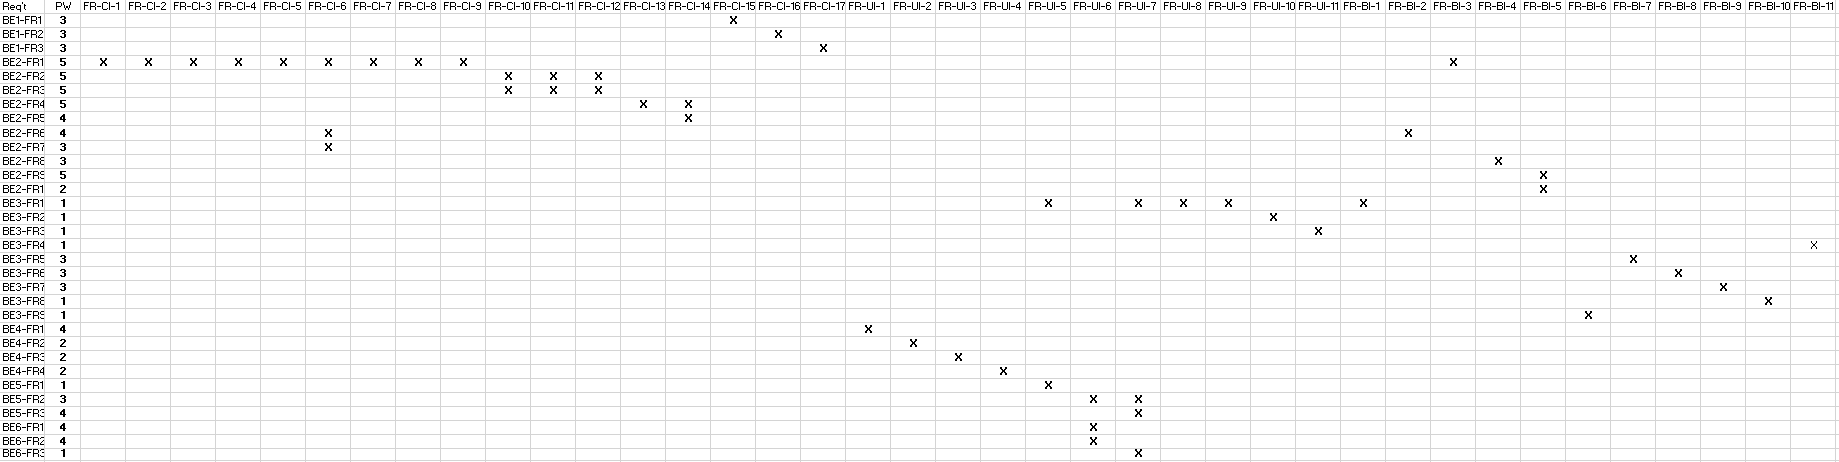
\includegraphics[width=1.2\textwidth]{TESTPLAN/traceabilitymatrix1.png}
		\caption{Traceability Matrix Fig.1}
		\label{fig:tm1}
	\end{figure}
	
	
	\begin{figure}[H]
		\centering
		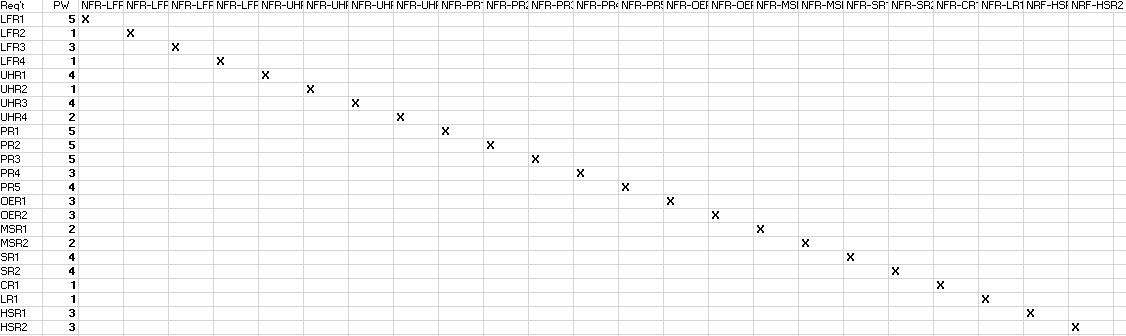
\includegraphics[width=1.2\textwidth]{TESTPLAN/traceabilitymatrix2.png} 
		\caption{Traceability Matrix Continued}
		\label{fig:tm2}
	\end{figure}
	
	
	\section{Tests for Proof of Concept}
	
	\subsection{Multiplayer}
	
	\paragraph{Multiplayer Test}
	
	\begin{enumerate}[{POC-}1. ]
		
		\item
		
		\textbf{Type:} Dynamic, Manual
		
		\textbf{Initial State:} Multiplayer Game active with 2 users
		
		\textbf{Input:} Tetromino movement command
		
		\textbf{Output:} For User 2: There must be displayed on screen two different boards one which is not controlled by user 2 and which shows the movement of user 1's Tetromino.
		
		\textbf{How test will be performed:} User will manually open 2 clients and connect to a multiplayer game. user will then input keystrokes to move a Tetromino in one client which observing if it moves in the other client.
		
	\end{enumerate}
	
	\subsection{User Interface and Gameplay}
	\paragraph{User Interface Test}
	\begin{enumerate}[{POC-}2. ]
		\item
		
		\textbf{Type:} Dynamic, Manual
		
		\textbf{Initial State:} Active Single player game
		
		\textbf{Input:} Tetromino movement command right
		
		\textbf{Output:} The Teteromino will move right one unit
		
		\textbf{How test will be performed:} User will manually start a game and press the keys to move the tetromino and verify the result.
	\end{enumerate}
	
	\paragraph{Gameplay Test}
	\begin{enumerate}[{POC-}3. ]
		\item
		
		\textbf{Type:} Dynamic, Manual
		
		\textbf{Initial State:} Active Single player game
		
		\textbf{Input:} Movement commands to cause a full row of spaces to be occupied by tetrominos.
		
		\textbf{Output:} The row will be removed from the board, the above rows will be lowered by 1 space and a new empty row placed on top.
		
		\textbf{How test will be performed:} User will manually start and cause the board to be in a state through movement commands where an entire row is occupied, then verify the results.
	\end{enumerate}
	
	
	
	\section{Comparison to Existing Implementation}	
	N/A No test plan is available for the current implementation				
	\section{Unit Testing Plan}
	Unit testing will be facilitated through the Jest framework.		
	\subsection{Unit testing of internal functions}
	To increase the efficiency of the testing process, we will use a hard-coded test oracle that encodes the expected results of the test cases as well as the code to set up the test cases. Once the test suite is run, the framework will indicate the whether the tests pass or fail, context about the failure as well as code coverage metrics. The results of the test will indicate where more developmental effort needs to be placed to increase the level of robustness. Additionally, the code coverage indicator will drive the placement of additional tests to get a higher level of coverage. Since games can be difficult to test, testing will be focused on aspects of the code that can be tested against an expected output. Therefore, only certain functions and methods will be able to be tested. That being said, the goal is to reach at least statement coverage for 85\% of the code.
	
	\subsection{Unit testing of output files}	
	Our system will not use unit testing of output files. Our system does not have any output files to test and creating some for the sake of testing seems like an inefficient use of development time. Instead of creating and unit testing output files, we will supplement with a more rigorous unit testing plan described above.
	\newpage
	\section{Appendix}
	
	This is where you can place additional information.
	
	\subsection{Symbolic Parameters}
	\begin{center}
		\begin{tabular}{|p{0.2\textwidth}|p{0.7\textwidth}|}\hline
			\textbf{SYMBOLIC CONSTANT} & \textbf{MEANING }\\\hline
			FR-CI & Functional Requirement - Controller Input  \\\hline
			FR-UI & Functional Requirement - User Interaction  \\\hline
			FR-BI & Functional Requirement - Board Interactions  \\\hline
			NFR-LFR & Nonfunctional Requirement - Look \& Feel Requirement  \\\hline
			NFR-UHR & Nonfunctional Requirement - Usability \& Humanity Requirement  \\\hline
			NFR-PR & Nonfunctional Requirement - Performance Requirement  \\\hline
			NFR-OER & Nonfunctional Requirement - Operational \& Environmental Requirement  \\\hline
			NFR-MSR & Nonfunctional Requirement - Maintainability \& Support Requirement  \\\hline
			NFR-UHR & Nonfunctional Requirement - Security Requirement  \\\hline
		\end{tabular}
	\end{center}
	\subsection{Usability Survey Questions}
	\begin{itemize}
		\item On a scale from 1-10, how would you rate the modernity and appeal of the game's graphics? 
		\item Are you satisfied with the performance of the game on your computer?
		\item How long was your longest game session playing this game?
		\item Would you recommend Tetris Tussle to a friend?
		\item Did you enjoy playing the game?
		\item How does this version of Tetris align with your expectations?
		\item Were the graphical elements easy to see/read?
		\item On a scale from 1-10, how easy was this game to play?
		\item What improvements would you make to this game?
		\item Was the user interface intuitive in your opinion?
	\end{itemize}
	% This is a section that would be appropriate for some teams.
	
\end{document}